\documentclass{article}
\usepackage[margin=1in]{geometry} % Set margins.
\usepackage{authblk} % Better formatting of affiliations.
\usepackage{url} % Allow URLs.
\usepackage{graphicx} % Allow figures.
\usepackage{xcolor} % Allow colored text.

\title{The Percolator 3.6 Mass spectrometry data post processor}

\author[1]{Lukas K\"{a}ll}
\author[2,3]{William Stafford Noble}
\author[4]{Will Fondrie}
\author[1]{Markus Ekvall}
\author[5]{Matthew The}
\author[2]{Charles Grant}

\affil[1]{Science for Life Laboratory, KTH -- Royal Institute of Technology}
\affil[2]{Department of Genome Sciences, University of Washington}
\affil[3]{Paul G.\ Allen School of Computer Science and Engineering,
  University of Washington}
\affil[4]{Talus Biosciences}
\affil[5]{Chair of Proteomics and Bioanalytics, Technical University of Munich, 85354 Freising, Germany}

% For things that need to be fixed.
\newcommand{\fixme}[1]{\color{red}FIXME: #1\color{black}}

\begin{document}

\maketitle

\begin{abstract} 
This is a very abstract abstract.
\end{abstract}

\section{Introduction}

The Percolator algorithm, first described in 2007 \cite{kall:semi-supervised}, has become one of the most widely used software tools in the field of mass spectrometry proteomics.
The Percolator software takes as input database search results produced by any one of a variety of search tools and then applies a semi-supervised machine learning approach to rank the identified spectra based on the quality of the peptide-spectrum matches.

\section{Methods}

\section{Results}

\subsection{Speeding up Percolator}

We implemented two speedups in Percolator.
First, we incorporated a Windows-compatible version of conjugate
gradient least squares support vector machine training \cite{halloran:speeding}.
Second, we implemented a layer-ordered heaps sorting and selection
strategy for partitioning training sets \cite{lucke:performing}.

On an Intel-i5 9600K-3.7 GHz-6core cpu, we measure a performance increase of 89\% with the new code as compared to version 3.03 when processing a very large set of $2.5\cdot10^8$ peptide-spectrum matches (4.0 vs 2.1 CPU hours needed).
The performance increase is fairly consistent accross sizes of data sets, see Figure \ref{fig:performance}. The performace increase between Percolator 2.8 and 3.0 was implemented by allowing parallel processing, which lead to a lower requirement of overall processing time (``wall time'') but not on the amount accumulateed CPU time over all the process. However the performance increase from 3.3 to 3.6 lowers the requirements on wall time as well as the CPU time.  
The amount of needed RAM emmory is however, fairly consistent over the tested versions.
% $ more res/per.36.25000k.time 
% 7241.00user 318.48system 51:49.33elapsed 243%CPU (0avgtext+0avgdata 26727048maxresident)k
% 83856inputs+927880outputs (1major+351954695minor)pagefaults 0swaps
% $ more res/per.33.25000k.time 
% 14156.46user 108.39system 1:24:18elapsed 282%CPU (0avgtext+0avgdata 32813852maxresident)k
% 24inputs+136outputs (1major+130080852minor)pagefaults 0swaps

% (14156,46+108,39)÷(7241.00+318.48) = 1,887


\begin{figure}
  \begin{center}
    \begin{tabular}{ccc}
    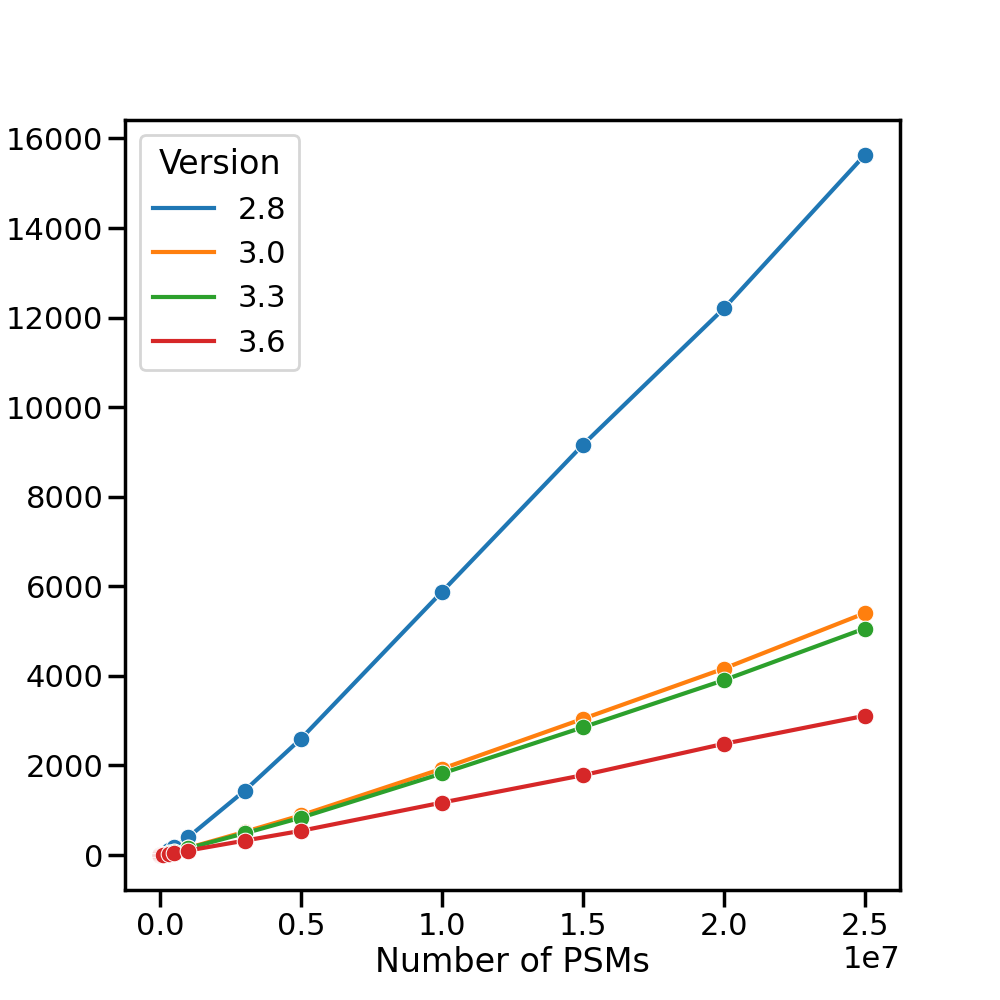
\includegraphics[width=0.3\linewidth]{img/wall.png} &
    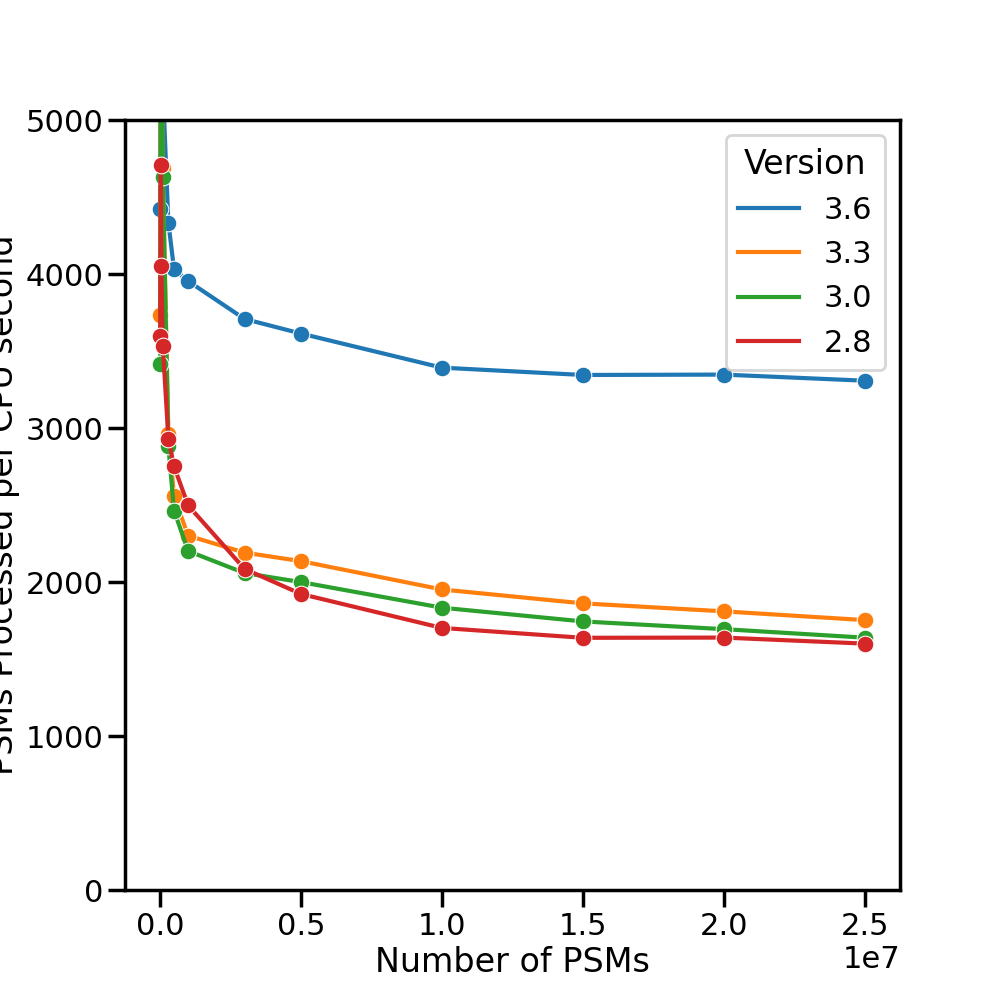
\includegraphics[width=0.3\linewidth]{img/rate.png} &
    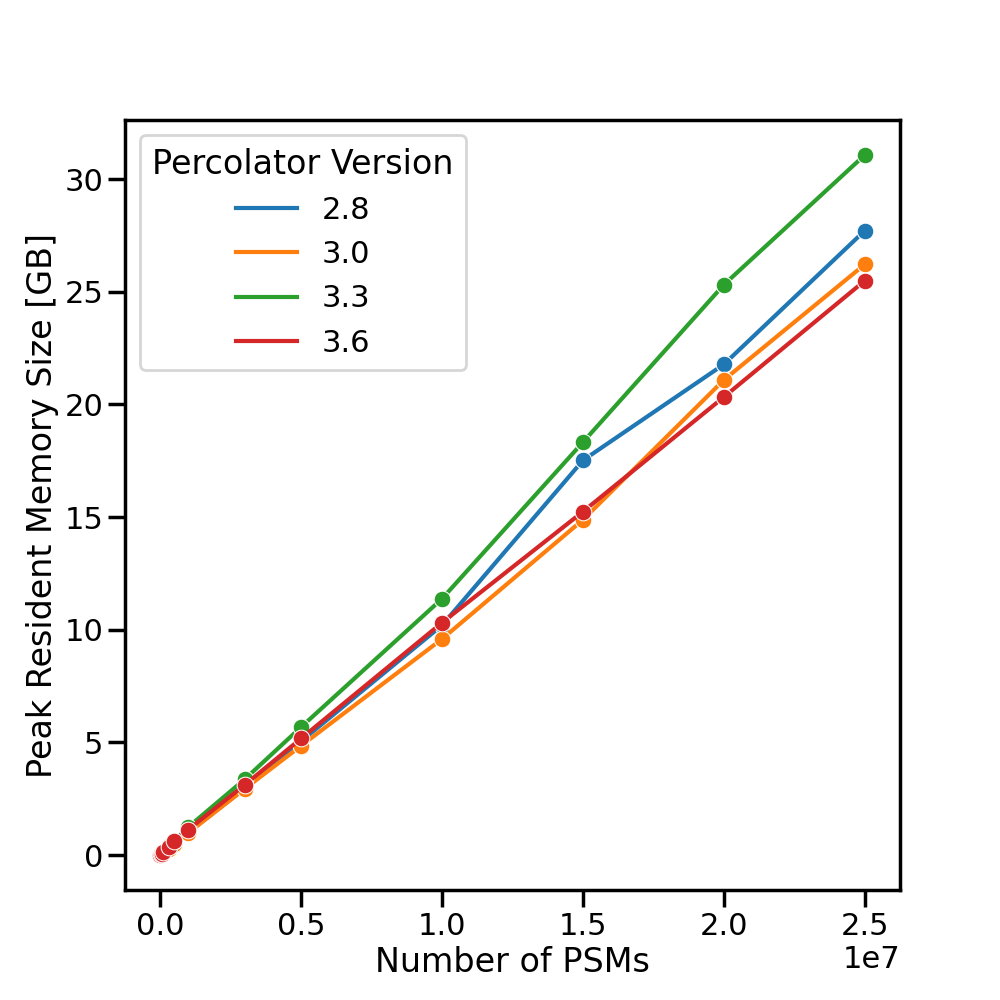
\includegraphics[width=0.3\linewidth]{img/memory.png} \\
    A & B & C \\
    \end{tabular}
    \caption{\textbf{Newer verions of Percolator uses less resources than older ones.} 
      The reduced demands by newer version of percolator as (A) the wall clock time as a function of the number of processed PSMs,
      (B) the number of PSMs processed per CPU second as a function of the number of PSMs, and
      (C) the peak resident memory size, i.e. the amount of RAM needed as a function of the number of PSMs. 
      For the plot we subsampled a set of 25 million PSMs, and executed the different verions of percolator 6 times and reported the execution with the lowest resource usage, to minimize the potential influence of other processes on performance.}
    \label{fig:performance}
  \end{center}
\end{figure}

\subsection{Integration with FragPipe}

Benchmark between fragpipe with Peptide Prophet and with Percolator?

We have implemented a protocol for using Percolator to match MS1 precursors accross different mass spectrometry runs based on their difference in mass and retention time \cite{the:focus}, which allows the software to be used for label-free quantification.

We have also implemented an interface to the OpenSWATH module EasyPQ, thereby facilitating using Percolator as a part of data-independent acquisition
workflows.

\section*{Methods}

We benchmarked the performance of Percolator ver 2.8, 3.0, 3.3, and 3.6 on an Intel-i5 9600K-3.7 GHz-6core cpu, downloaded from \url{https://github.com/percolator/percolator/releases}. The dataset used was 25 million PSMs, with spectra from Kim {\em et al.}\cite{kim2014draft} matched to uniprot with Crux\cite{park2008rapid}.
The runtime and memory use performance was measured with Linux's {\tt /usr/bin/time} command. 

\section*{Discussion}

Behind the scenes, we have also improved Percolator from a software engineering perspective.
First, we have implemented continuous integration of the Percolator source code via Github Actions.
This implementation automatically generates installation packages for Windows, MacOS, Ubuntu and CentOS.
Second, we have created extensive automated unit testing.
To do so, we have integrated the Google Test framework into the CMake build, as an optional feature.
The automated build system runs the unit test suite automatically with each check-in and includes support for the code coverage tool gcov.

\paragraph{Acknowledgements}

This work was supported by \fixme{get verbiage for CZI award.}

\bibliographystyle{plain}
\bibliography{percolator}

\end{document}
